\documentclass{llncs}
\usepackage{makeidx}
\usepackage{cite}
\usepackage{graphicx}
\usepackage{amssymb}

%

\begin{document}
\pagestyle{plain}

\mainmatter

\title{Accounting for Heterogeneity Across Multiple Imaging Sites Using Multi-Task
  Learning}
%
\titlerunning{short title}  % abbreviated title (for running head)
%
% use \inst{1} to get numbered tags on authors to match affiliations
\author{Michelle T. Hromatka\inst{1} \and Wei Liu\inst{1}  \and Jeffrey S. Anderson\inst{2} \and Brandon A. Zielinski\inst{3} \and Molly B. DuBray\inst{4} \and P. Thomas Fletcher\inst{1}}

\institute{School of Computing\and Division of Neuroradiology \and Division of Child Neurology\and
Interdepartmental Program in Neuroscience
\\ University of Utah, Salt Lake City, UT 84112, USA}

\maketitle

\begin{abstract}
Combining imaging data from multiple sites has the potential to increase
statistical power in clinical studies. However, while pooling multiple data
sources increases sample size, it also increases unwanted variance due to
inconsistencies across sites, e.g., different scanners, protocols, and
demographics. In this paper, we present an approach for combining multi-site
imaging data in classification tasks that takes this heterogeneity into
account. The idea is to treat the classification problem as a multi-task
learning problem, where each imaging site is treated as a ``task''. We employ a
regularized support vector machine (SVM) that allows for differences in decision
boundaries at individual sites, while at the same time leveraging the
similarities in the decision boundaries across sites. We demonstrate the
effectiveness of this approach in the classification of autism from multi-site
functional magnetic resonance imaging (fMRI) from the Autism Brain Imaging Data
Exchange (ABIDE). The proposed method achieves state-of-the-art accuracy and
outperforms a comparable SVM classifier applied to pooled data as well as
individual SVM classifiers applied per site.

% This paper combines traditional learning methods with regularized multi-task learning  to account for the differences between site data while still assuming similarity between tasks.  The ABIDE dataset is used for this research where a third of the data are removed and used to select a variety of parameters which are then used within a leave-one-out SVM classifier for the remaining test subjects. \keywords{SVM classification, ABIDE, Autism, ASD, multi-task learning, multi-site data }
\end{abstract}

\section{Introduction}
Recent years have seen a movement towards combining neuroimaging data collected
across multiple sites. Such multi-site data has the potential to accelerate
scientific discovery by increasing sample sizes, providing broader ranges of
participant demographics, and making data publicly available. Different
approaches include large, coordinated multi-site neuroimaging studies, such as
the Alzheimer's Disease Neuroimaging Initiative (ADNI) \cite{adni} as well as
data sharing initiatives that combine multiple single-site studies, such as the
Autism Brain Imaging Data Exchange (ABIDE) \cite{abide}. Analysis using these
datasets, however, is not straightforward, due to differences across site
scanners, protocols, populations, and diagnosis techniques. Treating a
multi-site study as a single, homogeneous data set fails to account for this
variability, which can be detrimental to the statistical power and counteract
the gains made by increasing the sample size.

In addition, many sites do not have a large enough sample size to use learning
algorithms on site-specific data.  Meta-analysis, in which results across small
studies are combined to extract patterns common in each, has previously been
used to combine site-specific results, especially when the sample size is low.
However, meta-analysis is not free of subjectivity of data variability, thus
this method of combined analysis is also faulty \cite{meta}.

Several groups have used the ABIDE dataset for classification with different, non-meta-analytic approaches. Nielsen, et al. combines the ABIDE dataset with a whole-brain approach, using a leave-one-out classifier to compute a classification score for each left-out subject based on age, gender and handedness.  The correlations for each connection in turn were fit with a linear model, separating controls from ASDs, which was then adjusted by the difference between the subject's site mean for that connection and the overall mean.  This approach yielded a maximum overall accuracy of 60.0\% despite finding significant positive correlation between the classification score and several of the phenotypic behavioral measures \cite{Jared}. A different study used histogram of gradients and applied this to several multi-site imaging studies which was able to achieve 61.7\% accuracy on the ABIDE dataset and 62.6\% on the ADHD-200 dataset \cite{ghiassian}. While \cite{Jared} accounted for some of the site differences, both studies approached the differences across imaging sites as noise instead of extra data that can be leveraged when classifying an aggregate data set.
This is the key principle in multi-task learning: heterogeneity across similar tasks can be accounted for while using a common mean to account for similarities between the different tasks.  This approach will be applied within an SVM classifier on the ABIDE dataset.

% Many researchers fail to take these differences as a****8, but rather as increased noise when treating with the drawback of increased noise due to scanner, protocol and population differences.}

\section{Methods}
Classification of multi-site imaging data can be thought of as a multi-task learning problem where each site,  $s$, is treated as a separate task, $t$.  For a dataset with $S$ sites, the corresponding multi-task problem will have a set of $T = S$ tasks and a function $F(t)$ that describes the relationship between each task.
Prior to using any sort of machine learning, however, nuisance factors (e.g. age) should be ***removed? from the data to ideally isolate differences across all data that are exclusive to the ***disease, disorder?**** being studied.

% SVM parameters through cross-validation and the features to be used in classification (see \ref{subsec:FS}).  These parameters are then used in a leave-one-out classifier on the testing data to determine the algorithm's accuracy, sensitivity and specificity. It is important to note that all parameter tuning and feature selection is done exclusively on the \textit{training} set, and the testing set is only used in the final classification to avoid inflation of results.

\subsection{Multi-Task Learning}
Evgeniou and Pontil (2004) introduces a method of multi-task learning based on kernel based methods typically used for single task learning.  This method relies on minimizing regularization functions, such as that for SVM, to capture both overall similarity between tasks and individual task differences.  The traditional minimization for a soft margin SVM is:\\
\begin{equation}
\label{eq:svm}
\frac{1}{2}w^2 + C F(\sum_{i=1}^t \xi_i)
\end{equation}
where $C$ is a constant and $F(\mu)$ is a "monotonic convex function with $F(0)=0$ \cite{svm}. In the case of SVMs, the weight vector $w$ is used to define the hyperplane, $(w \cdot x +b)$,  which is the boundary between groups.

For multi-task learning, the relationship between $T$ tasks must be described, which Evgeniou and Pontil approach using the hierarchical Bayes method. This assumes that each task function comes from a class of probability distributions.  The relationship is defined as:\\
\begin{equation}
\label{eq:sim}
 w_t = w_0 + v_t ,
\end{equation}
where $w_0$ is the mean of the data and each task $t$ has its own weight vector, $v_t$. Multi-task learning allows for simultaneous learning of the mean of all tasks, $w_0$, and each task weight vector, $v_t$, so the minimization function then becomes:\\
\begin{equation}
\label{eq:mtlsvm}
 C \sum_{t=1}^T \sum_{i=1}^m \xi_{it} + \frac{\lambda_1}{T} \sum_{t=1}^T ||v_t||^2 + \lambda_2||w_0||^2 ,
\end{equation}
where $\lambda_1, \lambda_2$ are "positive regularization parameters" and $C$ is still a constant.  For high similarity between tasks, the $v_t$ will be small in relation to $w_0$; this relationship is described by the hyperparameters $\lambda_1, \lambda_2$ that must be chosen by the user.

The dual of equation \ref{eq:mtlsvm} can be found by defining a set of functions $f_t(x) = w_t \cdot x$ which can be simplified to $F(x,t) = f_t(x)$.  This can be described by a kernel function $\phi((x,t))$ which allows us to relate the dual of a multi-task learning problem to the dual of Equation \ref{eq:svm}.
\begin{equation}
\label{eq:mtldual}
\max_{\alpha_{it}}  \left\{ \sum_{i=1}^m\sum_{t=1}^T \alpha_{it} -  \sum_{i=1}^m\sum_{s=1}^T\sum_{j=1}^m\sum_{t=1}^T  \alpha_{is}y_{is}\alpha_{jt}y_{jt}\phi((x,t))      \right\}
\end{equation}
where
\begin{equation}
\phi((x,t)) = \big(\frac{x}{\sqrt{\mu}}, \underbrace{0,...,0}_{t-1}, x, \underbrace{0,...,0}_{T-t} \big), \quad \textbf{for  } \mu = \frac{T\lambda_2}{\lambda_1} .
\end{equation}
As you can see in Equation \ref{eq:mtldual}, this is the same dual problem as for a single task-SVM, with the data transformed by $\phi((x,t))$ into the multi-task kernel space.




\subsection{Feature Selection}
\label{subsec:FS}
Data extraction in imaging studies typically leads to very high dimensional data spaces.  For f-MRI, a typical choice for data is the pairwise correlation between $n$ predefined regions of the brain.  This yields a dataspace of $\frac{n(n+1)}{2}$ dimensionality, which, even for a relatively small number of regions, can be  computationally expensive.  The multi-task learning above further increases dimensionality with the number of tasks. For a feature space $x \in \mathbb{R}^d$, the multi-task kernel $\phi((x,t))$ would yield a feature space of $d(t+1)$ dimensions.  Feature selection can and should be employed to remove redundancy and increase relevancy of the data while reducing computation time \cite{featsel}.

A ****** approach is to use a simple hypothesis test to determine which features would be most useful in classification.  Nuisance factors, such as age or ******, should be accounted for prior to the hypothesis test to ideally isolate differences attributed to the disease or disorder being studied.  A linear model is then fit to the training set one feature at a time based on group.  If the coefficient for the group  has a $p < .001$, the feature is kept and used in the SVM classification. This test is done on each feature in turn, ultimately reducing the data into a set that has significant differences between groups.
\section{Evaluation}
\subsection{Data}
The Autism Brain Imaging Data Exchange(ABIDE) database is an online consortium of resting-state functional-MRI data from 17 international sites, resulting in brain imaging data for 539 individuals with ASD and 573 typically developing(TD)  controls \cite{abide}. All ASD subjects were diagnosed by either the Autism Diagnosis Observation Schedule-General(ADOS-G) or the Autism Diagnostic Interview-Revised tests and removed from the study if other co-morbid disorders were present \cite{lordADOS} \cite{lordADIR} \cite{abide}.  Further inclusion details can be found at (put url? citation to... website? or the abide paper?)
\subsubsection{Preprocessing}
All data was preprocessed using the Functional Connectomes-1000 preprocessing scripts \cite{fcon}. This includes:
\begin{enumerate}
\item MRI Deoblique, reorient, skull strip
\item f-MRI Reorient, motion correct, skull strip, smooth
\item registration
\item Segmentation - csf, white matter
\item extracting global signal, from csf and wm
\item extract time series, Z-transform correlations
\item spatial smoothing, register to atlas
\item some sort of regression
\end{enumerate}
Twelve subjects were removed because of failure during the preprocessing.  Two Oregon subjects were missing the resting fMRI file and 10 UCLA subjects were missing the anatomical scan file which is required in step 1 of the preprocessing pipeline above. This resulted in 1100 subjects for analysis, 530 ASD and 570 TD controls.
\subsubsection{Data Extraction}
From each subject's postprocessed image, the time series for each of 264 regions is extracted based on Power's regions of interest \cite{Powers}. These 264 regions are spread out among the cerebral cortex, subcortical structures and cerebellum, where each region is a sphere of 5mm in radius and regions are separated by a minimum distance of 10mm so as to avoid detection of a shared signal. The Fisher transformed Pearson correlation coefficient is then found between each region and the other 263 regions, resulting in a 34,716 dimensional feature space for each subject. After feature selection, this number is reduced to 312 features per subject.
***add in featsel, multiplication/interdependence of features??
\subsection{Results}

\section{Discussion and Conclusion}
\begin{figure}
	\centering
	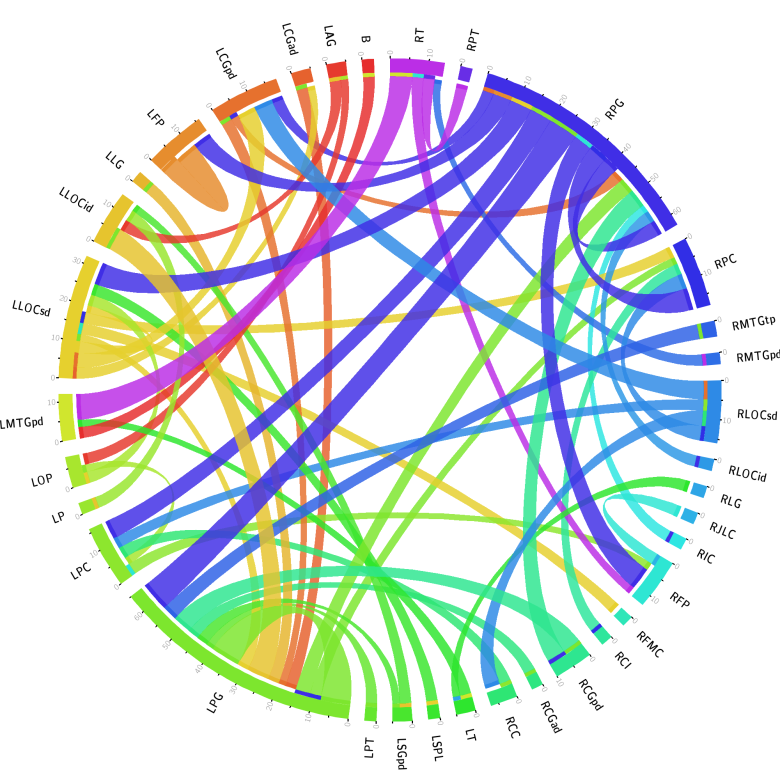
\includegraphics[scale = .3]{now_circos.png}
	\caption{The pairwise connections, represented as ribbons connecting each region, selected by the hypothesis test described in \ref{subsec:FS}.  The width of each ribbon is determined by the weights from the $w_0$ vector in the SVM. }
	\label{fig:circos}
\end{figure}


\bibliography{miccai}{}
\bibliographystyle{plain}





\end{document}